% Chapter X

\chapter{Simulating Collisions in Thermal Gases} % Chapter title

\label{ch:inhomogas} % For referencing the chapter elsewhere, use \autoref{ch:inhomogas} 

%----------------------------------------------------------------------------------------

Need to introduce the usefulness of the method here. References to many kinds of applications and such things. I also need to perform a literature review of all DSMC used in cold atoms physics.

Compare to molecular dynamic approaches, when is DSMC appropriate / good? When does it fail? 

Find out the knudsen number for typical cold atom conditions. Wade has numbers for stamper kern and shvatchuck.

DSMC - Birds Book \cite{Bird1994}

Evaporative Cooling and Expansion Dynamics: \cite{Wu1996, Wu1997, Wu1998}

Bosonic Collective-Mode dynamics: \cite{Jackson2001, Jackson2001b, Jackson2002, Jackson2002b, Jackson2002c}, Can't find Jackson Zaremba 2002 Laser Physics, 12, 93

Fermion Dynamics: \cite{Urban2006, Urban2007, Urban2008, Lepers2010} (see also \cite{Vignolo2002, Toschi2003, Capuzzi2004, Toschi2004})

Sympathetic Cooling: \cite{Barletta2010, Barletta2011}

Applications - Rayleigh Bernard Flow: \cite{Watanabe1994}

Spacecraft aerodynamics: \cite{Oran1998}

Chemical reactions: \cite{Anderson2003} Goldsworthy?

Microfluidics: \cite{Frangi2003}

Acoustics on Earth, Mars and Titan: \cite{Hanford2009}

Volcanic plumes on Jupiter: \cite{Zhang2004}

Read: \sout{\cite{Minguzzi2004}}, [45]

Refer to cuda section \ref{ch:cudadsmc} Should also discuss the development of this parallel implementation of the code. Compare to CPU implementations. Goldsworthy has a few references for other CUDA codes.

The heart of the DSMC method is to simplify the simulation of interparticle interactions in the form of two body collisions.
In this sense there are two aspects we need to ensure are modelled accurately; the number and frequency of collisions (collision rate) and the collisions themselves, wether or not they are correctly distributing the kinetic energy.
In the following sections I carefully analyse these two aspects to ensure the utmost accuracy in our simulations.

%----------------------------------------------------------------------------------------

\section{Collision Rates in Thermal Gases} \label{sec:collisionRates}

Overall collision rate, spatial collision rate, talk about number of cells, the occupancy of cells and the effect of inhomogeniety.
 
One of the most basic tests of the application of the DSMC method to cold atom physics is to investigate the collision rate for a thermal gas.
\marginpar{Maybe say something about the Boltzmann equation here and give some references.} 
Using the Boltzmann equation we can derive \cite{Walraven2010} the thermally averaged collision rate per unit density for a single species atomic gas bound by the potential ${\cal U}(\mathbf{r})$,
\begin{equation}
    {\tau_c}^{-1} = \frac{1}{2} n_{0}\langle v\sigma \rangle \frac{V_{2e}}{V_e},
\end{equation}
where $n_0 = N / V_e$ is the central density of the gas, $\langle v\sigma \rangle$ is the thermally averaged product of the atomic velocity and collision cross section, \\*$V_e = \int \exp\left[-{\cal U}(\mathbf{r})/kBT\right]\, d\mathbf{r}$ is the effective volume of the gas, and \\*$V_{2e} = \int \exp\left[-2{\cal U}(\mathbf{r})/kBT\right]\, d\mathbf{r}$ the effective volume corresponding to the distribution of pairs.
\marginpar{ The effective volume, $V_e$, of an inhomogeneous gas equals the volume of a homogeneous gas with the same number of atoms and density. }
For the bulk of this work we will consider collisions in three unique trapping potentials: no trapping potential, \ie  a homogeneous gas, an Ioffe Pritchard trap(cite) and a spherical quadrupole trap(cite - is it really spherical?)\footnote{We have a more in depth discussion of magnetic trapping in appendix \ref{sec:magneticTrapping}.}. 
In table \ref{tab:collisionrates} we have derived the expressions for the effective volume and average collision rates for each of these traps. We have also included the results for a general isotropic power law trap, the potential of which is described by
\begin{equation}
    {\cal U}_{\mathrm{PL}}(\mathbf{r}) = {\cal U}_0 \left(\frac{\mathbf{r}}{r_e}\right)^{3/\gamma}, \label{eq:powerlaw}
\end{equation}
where the trap has a characteristic trap size $r_e$ and a trap strength of ${\cal U}_0$. The parameter, $\bar{v}$, in table \ref{tab:collisionrates} is the thermally averaged atomic speed and is given by
\begin{equation*}
    \bar{v} = \sqrt{\frac{8 k_B T}{\pi m}}.
\end{equation*}

\begin{table}
\hspace{-16em}
\myfloatalign
\begin{tabularx}{1.35\textwidth}{|l|c|c|c|} \toprule
\tableheadline{Trapping Potential} & \tableheadline{Trap Power} & \tableheadline{Effective Volume, $V_e$} & \tableheadline{ Collision Rate, ${\tau_c}^{-1}$} \\ \midrule
Homogeneous Gas & $\infty$? &  V & $\frac{1}{2^{1/2}}n_0\bar{v}\sigma$ \\
\midrule
Spherical Quadrupole & 1 & $256\pi\left(\frac{ k_B T}{g_s \mu_B B_z}\right)^3$ & $\frac{1}{2^{7/2}}n_0\bar{v}\sigma$ \\
\midrule
Ioffe Pritchard & 2 & $\frac{8}{\sqrt{B''}B_\rho''}\left(\frac{ \pi k_B T}{g_s \mu_B}\right)^{3/2}$ & $\frac{1}{2^2}n_0\bar{v}\sigma$ \\
\midrule
Isotropic Power Law & $3/\gamma$ & $\frac{4}{3}\pi{r_e}^3\Gamma\left[\gamma+1\right]\left(\frac{k_B T}{{\cal U}_0}\right)^{\gamma}$ & $\frac{1}{2^{\gamma+0.5}}n_0\bar{v}\sigma$\\
\bottomrule
\end{tabularx}
\caption[Collision rates for different trapping potentials.]{Collision rates for different trapping potentials.}  
\label{tab:collisionrates}
\end{table}

We can make a few interesting observations from these calculations. The most interesting is that the collision rate in the trapped gases \emph{increases} as the temperature \emph{decreases}, which is the converse to the homogeneous gas\footnote{This relationship between collision rate and temperature for trapped gases is what gives rise to the "runaway" evaporation observed during atom cooling experiments.}. 
This is because for a trapped gas the central density increases at a rate greater than the decrease of the average thermal velocity, $\bar{v}$. 
For the homogeneous gas the density remains constant as the gas cools, thus the decrease in the velocity of the atoms results in an overall decrease in the collision rate.
We can also see that if we can hold the trap strength and effective trap size constant the central density of the trap will increase as the power of the trap decrease (or as $\gamma$ increases). 
This is often spoken about in terms of "tightness" and is a strong motivator behind the use of the quadrupole trap.
In section \ref{sec:evaporation} we will show that it is the tightness of a trap that determines it's efficiency in evaporative cooling.

%----------------------------------------------------------------------------------------

\section{DSMC simulations of collisions}

The DSMC method offers some free parameters which we can optimise to balance the accuracy and efficiency of the algorithm, namely the number of cells, $n_c$, and the number of test particles, $N_p$.
We wish to see the effect of varying these parameters on the results of the simulation.

**Include a surface plot of the collision rate as a function of cell number and test particle number.
Should make the z axis percentage error. See fig 14. in wade. **

\begin{figure}
\hspace{-8em}
\makebox[1.8\linewidth][l]{%
\centering
\subfloat[Homo err]{\label{fig:a}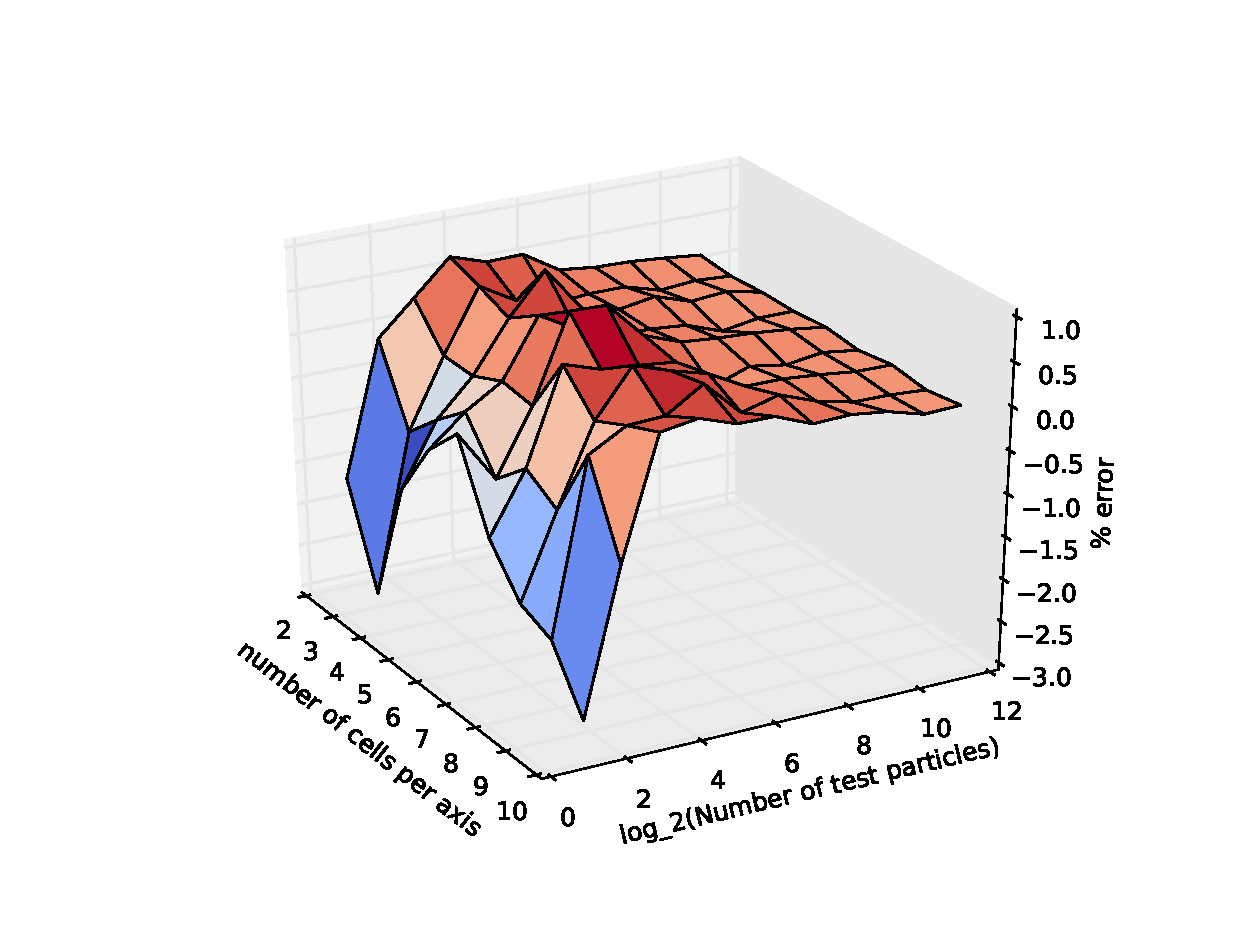
\includegraphics[width=0.525\textwidth]{gfx/HomoError}}%
\subfloat[IP err]{\label{fig:b}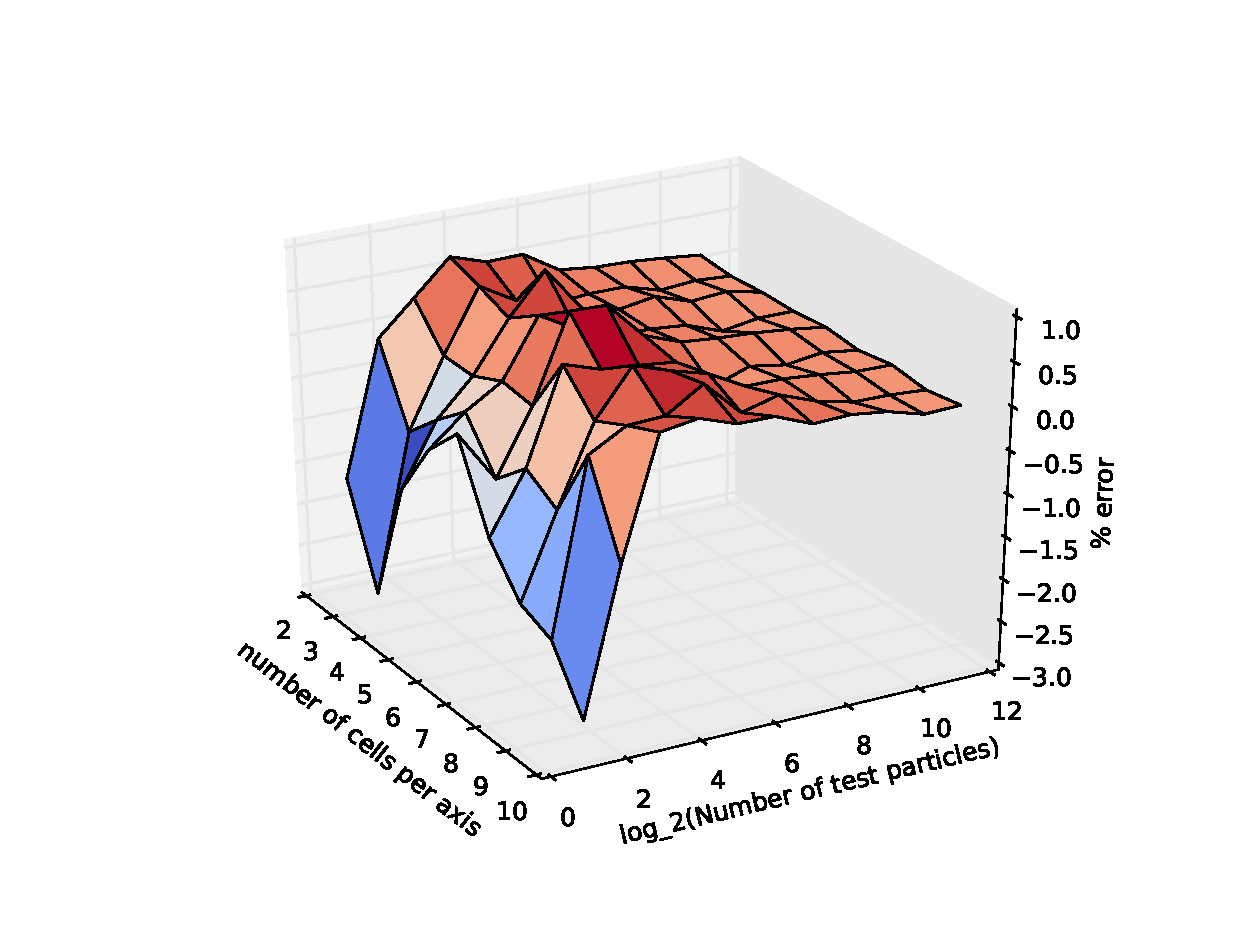
\includegraphics[width=0.525\textwidth]{gfx/HomoError}}%
\subfloat[Quad err]{\label{fig:c}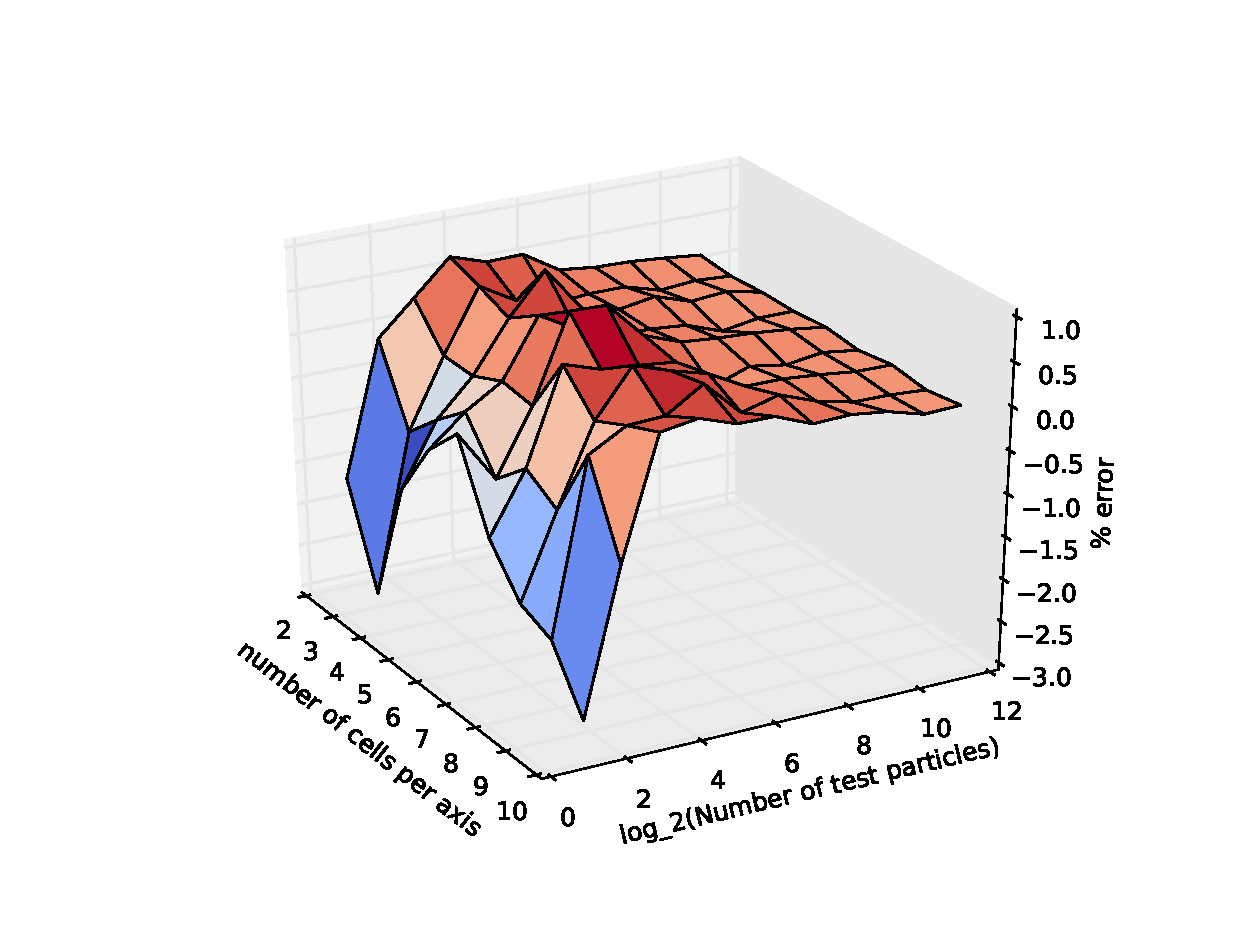
\includegraphics[width=0.525\textwidth]{gfx/HomoError}}%
}
\caption{Error of DSMC method as a function of test particle number and cell number.}\label{fig:dsmccolerr}
\end{figure}

Figure \ref{fig:dsmchomoerr} shows how well the DSMC method performs over a wide range of test particle and cell numbers in a homogeneous gas. 
We can see in the corner the method beginning to fail. 
This is the region where, on average, we have less than two test particles per cell. 
This means that there is not enough atoms to perform a collision within a cell. 
One way to avoid this (which has not been implemented here) is to search neighbouring cells for collision pairs when a partner can not be found in the current cell.
The main thing to observe here is the increase in the error as the number of test particles is reduced.

Smaller cells -> larger fluctuations.

Not adaptive since slowly changing cloud.


%----------------------------------------------------------------------------------------

\section{Thermalisation} 

Once we are convinced that we have the correct number of collisions we must confirm that they are performing as they should.
The perfect way to test this is through the investigation of \emph{thermal relaxation} or the process of thermalisation through elastic collisions.
\marginpar{Thermalisation is the generic name for all kinds of processes giving rise to relaxation towards thermal equilibrium starting from a non-equilibrium situation. **REWORD, NOT MY WORDS**} 
There are many ways that a system can be out of equilibrium, but here we will investigate three scenarios from the literature that have a concrete theoretical backing to which we can compare our simulations.

\subsection{Walraven Thermalisation} \label{sec:walravenTherm}

The simplest example for rethermalisation is somewhat reminiscent of evaporative cooling, that is the case is simply perturbing the equilibrium by adding a small number of atoms whose average energy is different to that of the bulk gas.
In \cite{Walraven2010} (the analysis of which we step through in detail in appendix \ref{app:walravenTherm}) we are shown that the rethermalisation time, ${\tau_{\mathrm{th}}}^{-1}$, is given by
\begin{equation}
    \tau_{\mathrm{th}}^{-1} = \frac{1}{2\left(\gamma + 3/2\right)} \tau_{c}^{-1}. \label{eq:walravenRetherm}
\end{equation}
If we use the values for the trapping parameter, $\gamma$, given in table \ref{tab:collisionrates} we would expect the thermalisation time in a homogeneous, IP and quadrupole trap to be 3, 6 and 9 times the collision time in each trap respectively.
Anderlini and Gu\'ery-Odelin \cite{Anderlini2006} have taken this analysis one step further, considering the effect including all partial waves in the collision integrals has on a homogeneous box trap and a harmonic potential.
Interesingly in the limit of constant cross section the results for the homogeneous trap reduces to that given in equation \eqref{eq:walravenRetherm} with $\gamma=0$.
In fact they go on to show that for the harmonic trap the thermalisation time is longer by a factor of 2, which again, agrees with equation \eqref{eq:walravenRetherm} with $\gamma=3/2$.

Before we consider these simulations numerically the reader might be a little confused by the above result. 
Looking at equation \ref{eq:walravenRetherm} it is quite clear that as the trapping parameter, $\gamma$, increases the number of collision required for thermalisation increases.
This might be a little counter intuitive.
We just stated in section \ref{sec:collisionRates} that evaporative cooling, a process driven by rethermalisation is more efficient in tighter trapping potentials \ie larger trapping parameters.
Aderlini et al. explain this best when they say
\begin{displayquote}
    \dots the fact that the space of configuration is larger for a nonhomogeneous gas, and that the thermalization affects both the space and velocity degrees of freedom.
\end{displayquote}
We can understand this better if we consider an effective volume in configuration space, $V_{cs}$, (analogous to the effective volume in real space, $V_{e}$)
\begin{equation}
    V_{cs} = \int \exp\left[ -\frac{H( \mathbf{r}, \mathbf{v})}{k_B T}\right]\,d\mathbf{r}d\mathbf{v} = V_e \left(\frac{3\pi m}{k_B T}\right)^{3/2}.
\end{equation}
So we can see that for a given temperature the region occupied in configuration space increases with the effective volume, which table \ref{tab:collisionrates} shows increases with $\gamma$.
Again this might make the reader uncomfortable, we seem to have convincigly shown that tighter trapping potentials take longer to thermalise. 
However, even though the number of collisions required to thermalise the gas increases with the trapping parameter, $\gamma$, the average time between collisions, $\tau_c$, decreases.
Thus the absolute time required for a gas to thermalise is lower for tighter trapping potentials \ie larger $\gamma$.

\begin{figure}
\hspace{-8em}
\makebox[1.8\linewidth][l]{%
\centering
\subfloat[Walraven homegeneous gas thermalisation. $\tau_{c}^{-1} / \tau^{-1} = 1.2$ should equal 3?]{\label{fig:walravenHomo}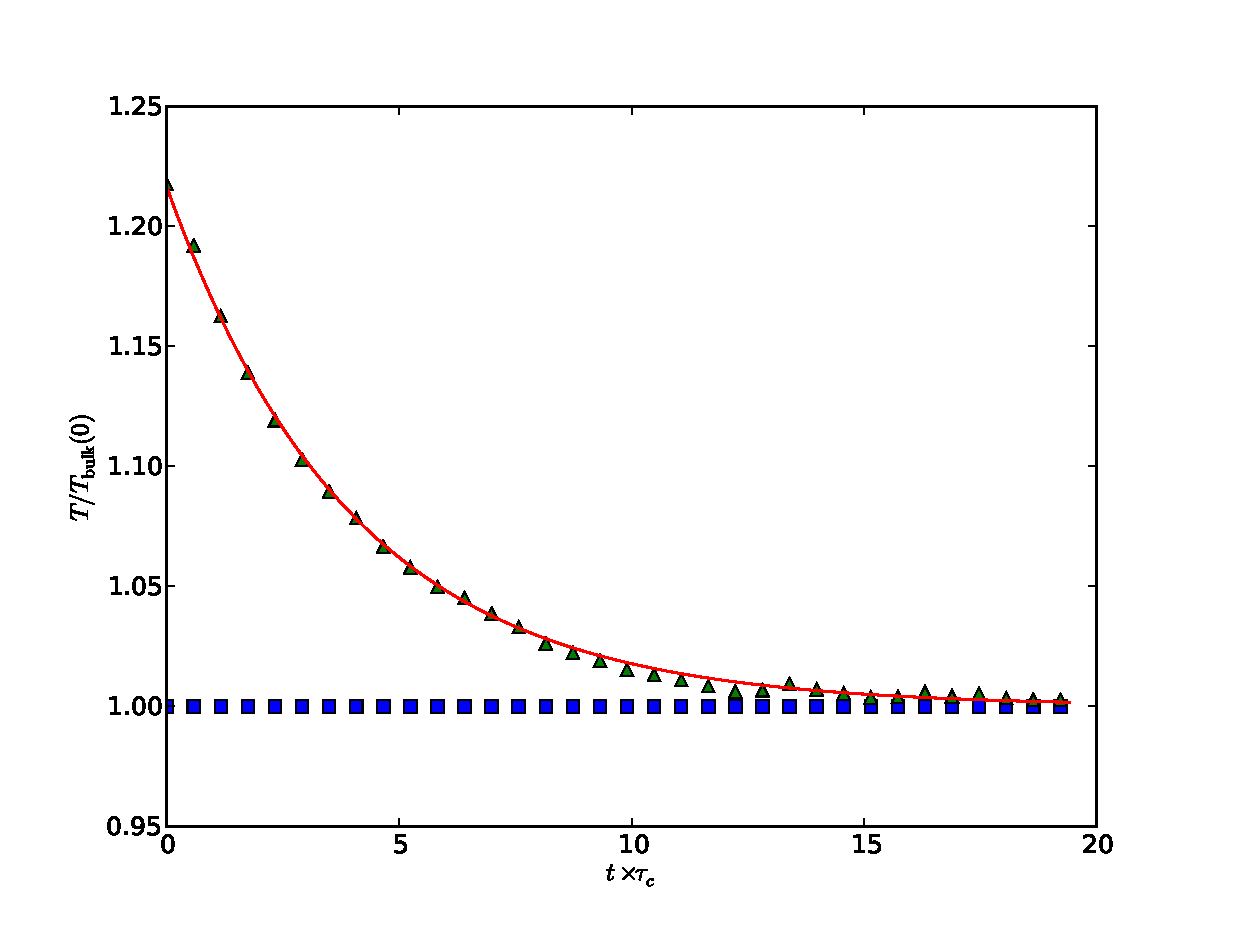
\includegraphics[width=0.525\textwidth]{gfx/Thermalisation/walravenHomo}}\quad
\subfloat[Walraven ip gas thermalisation. $\tau_{c}^{-1} / \tau^{-1} = 1.6$ should equal 6?]{\label{fig:walravenIP}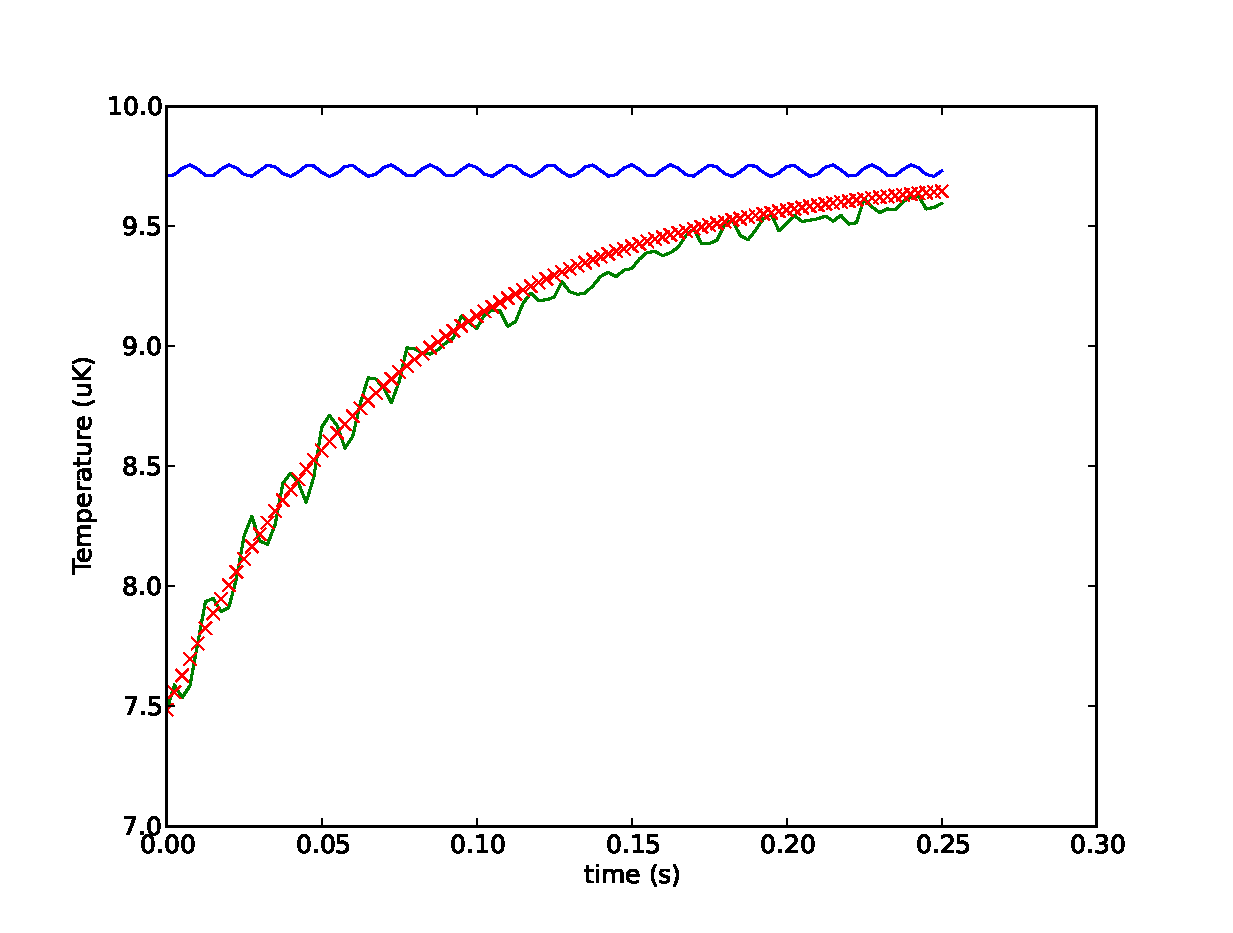
\includegraphics[width=0.525\textwidth]{gfx/Thermalisation/walravenIP}}\quad
\subfloat[Walraven quad gas thermalisation. $\tau_{c}^{-1} / \tau^{-1} = 10.45$ should equal 9?]{\label{fig:walravenQ}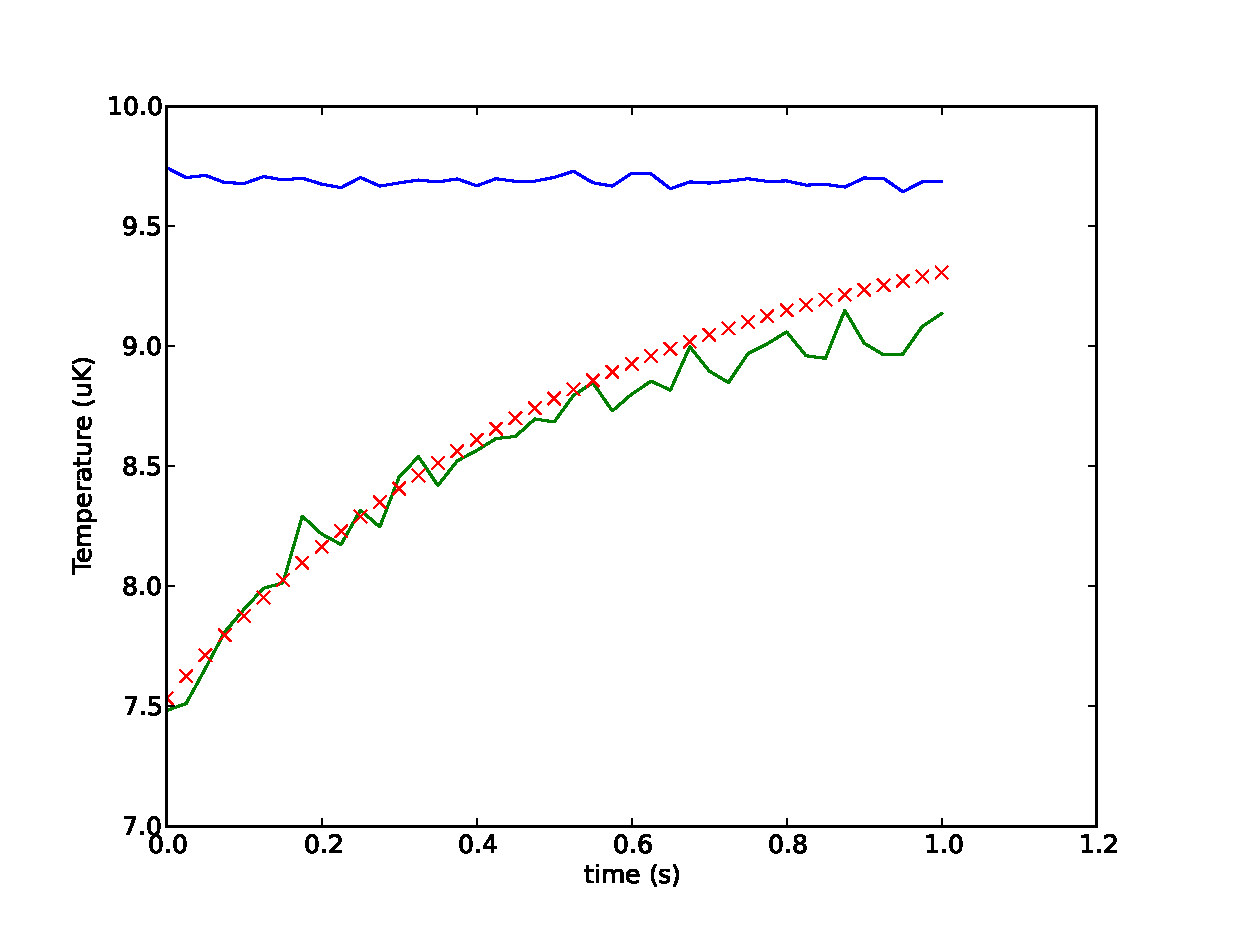
\includegraphics[width=0.525\textwidth]{gfx/Thermalisation/walravenQuad}}%
}
\caption{Walraven rethermalisation. I want to do this simulation for some different perturbation temperatures. One more higher and one lower too.}\label{fig:walravenTherm}
\end{figure}

In figure \ref{fig:walravenTherm} we have simulated a million physical atoms, $N_P=10^6$, at $10\,\mu \mathrm{K}$ in three different trapping potentials: homogeneous, IP and quadrupole. 
Each gas began in an initially thermal distribution with 10\% of the particles at set to have an average temperature of $12.5\,\mu\mathrm{K}$.
\marginpar{When choosing the initial perturbed distribution we must keep in mind the virial theorem \cite{}. The key result here is that in a thermal distribution we have $\langle E_p \rangle = \frac{2\gamma}{3} \langle E_k \rangle = \gamma k_B T$. So when choosing the width for the spatial distribution we must keep in mind the effective power of the trapping potential. }
For each simulation we have chosen the trapping parameters such that the collision rate was approximately 25 collisions per atom per second, as this number is similar to atoms of this temperature in an evaporation experiment.
We used one million test particle, $N_T=10^6$, in each simulation so that the ratio of physical atoms to test particles was one, $\alpha=1$.

For the homogeneous gas simulation shown in figure \ref{fig:walravenHomo} I set the width of the box containing the atoms to be $100\,\mu \mathrm{m}$ in each direction. 
This corresponds to a collision rate of $24.64\,\mathrm{s}^{-1}$.
I found the thermalisation occurred in $3.14\pm 0.02$ collision times, closely resembling the result in equation \eqref{eq:walravenRetherm}.

For the Ioffe Pritchard trap simulation shown in figure \ref{fig:walravenIP} we set $B_0=0.01\,\mathrm{T}$, $B'=33.54\,\mathrm{Tm}^{-1}$ and $B''=75,000\,\mathrm{Tm}^{-2}$ which equates to a ${B_{\rho}}''=75,000\,\mathrm{Tm}^{-2}$. 
Choosing these trapping parameters gives a collision rate of $24.72\,\mathrm{s}$.
I found the thermalisation occurred in $6\pm 0.1$ collision times, again, in perfect agreement with equation \eqref{eq:walravenRetherm}.

Finally in the quadrupole trap simulation shown in figure \ref{fig:walravenQ} we set $B_z=2.8\,\mathrm{Tm}^{-1}$ resulting in a collision rate of $25.48\,\mathrm{s}$.
I found the thermalisation occurred in $9\pm 0.1$ collision times, again, in perfect agreement with equation \eqref{eq:walravenRetherm}.

We can note from all simulations shown in figure \ref{fig:walravenTherm} that the thermalisation time appears to be independent of the size of the perturbation.

\subsection{Monroe Thermalisation}

Another interesting experiment that has been investigated in some depth is the rethermalisation of a directional anisotropy. 
In these experiments the kinetic energy is changed in one cartesian direction only (the spatial distribution is reshaped accordingly), creating a directional anisotropy in the distribution.
This squeezed distribution is then allowed to rethermalise through elastic collisions.
The original theoretical development of Myatt \cite{Myatt1997} predicts that in an harmonic trap the thermalisation time for a directional anisotropy is approximately 2.7.
This result has been used to experimentally determine the collision cross section, $\sigma$, of atoms in ultra-cold gas experiments \cite{Monroe1993, Davis1995}. 
This simulation has also been repeated by Wu and Foot \cite{Wu1996} using the DSMC method.
Here I have extended this investigation to consider the thermalisation times in our three favourite trapping potentials: homogeneous, Ioffe Pritchard and quadrupole.
As we saw in section \ref{sec:walravenTherm} we can't expect the thermalisation time to be the same in different trapping potentials.
In fact, if the perturbation is kept the same, it was purely a function of the trapping parameter, $\gamma$.

\begin{figure}
\hspace{-12em}
\makebox[1.8\linewidth][l]{%
\centering
\subfloat[Monroe homegeneous gas thermalisation. $\tau_{c}^{-1} / \tau^{-1} = 0.77$]{\label{fig:monroeHomo}\includegraphics[width=0.525\textwidth]{gfx/Thermalisation/monroeHomo}}\quad
\subfloat[Walraven homegeneous gas thermalisation. $\tau_{c}^{-1} / \tau^{-1} = 2.21$]{\label{fig:monroeIP}\includegraphics[width=0.525\textwidth]{gfx/Thermalisation/monroeIP}}\quad
\subfloat[Walraven quad gas thermalisation. $\tau_{c}^{-1} / \tau^{-1} = 6.09$]{\label{fig:monroeQ}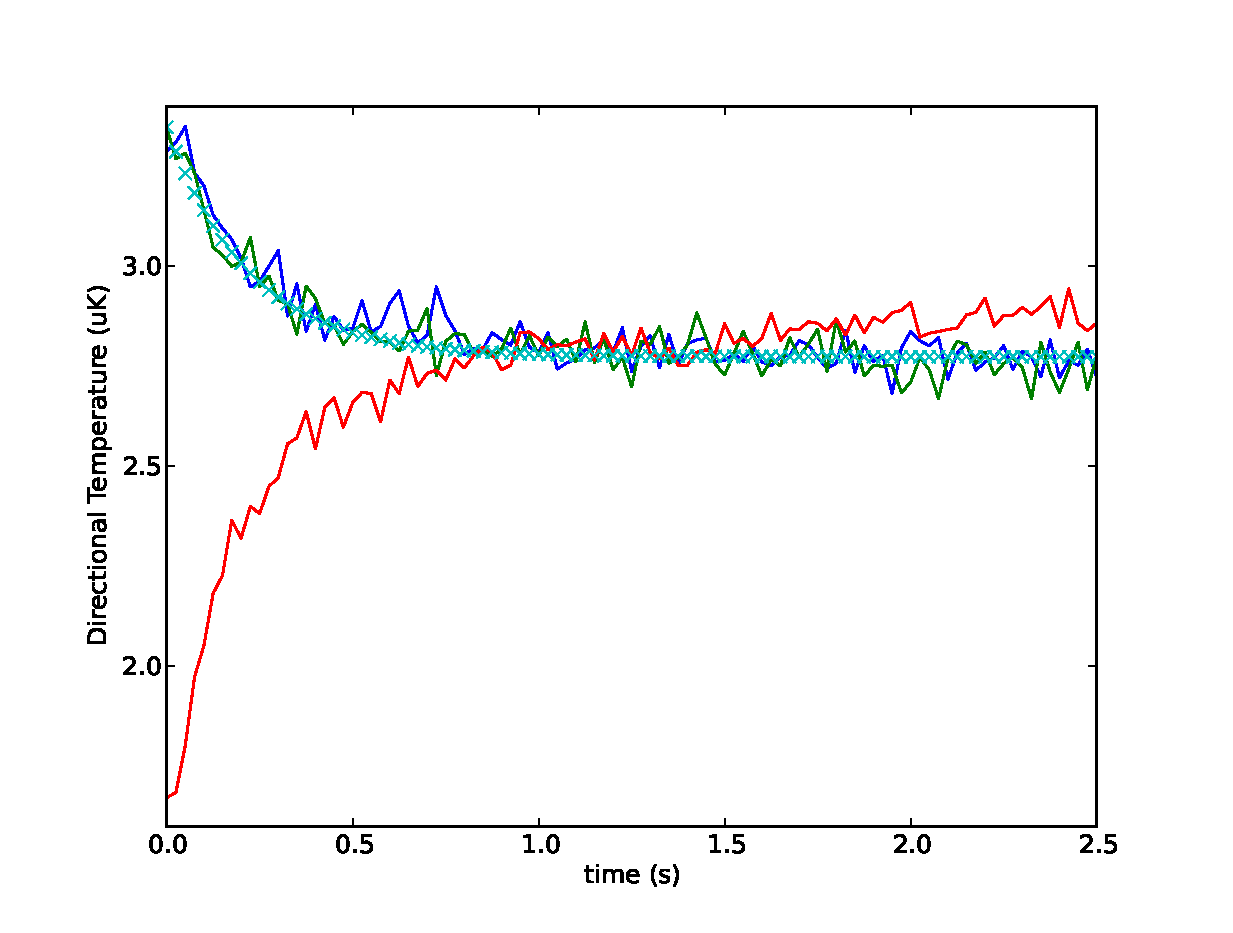
\includegraphics[width=0.525\textwidth]{gfx/Thermalisation/monroeQuad}}%
}
\caption{Walraven rethermalisation. I want to do this simulation for some different perturbation temperatures. One more higher and one lower too.}\label{fig:monroeTherm}
\end{figure}
Also do it for different temperatures or trap numbers.

*** MUST REDO ALL OF THESE SIMULATIONS WITH COLLISIONS WORKING CORRECTLY (I.E. WITH THE NEW SORTING FIX IMPLEMENTED). ***
\marginpar{Comment on directional temperatures being a useful tool for checking that collisions are working effectively. }
%----------------------------------------------------------------------------------------

\section{Evaporation} \label{sec:evaporation}

Compare some results to those predicted by the theory of walraven \cite{Walraven2010} and the other guy \cite{Luiten1996} . 

As demonstrated by Wu et al \cite{Wu1996, Wu1997} we can use the DSMC method to simulate evaporative cooling.
There has been a lot of theoretical investigation into the evolution of cold gases under forced evaporative cooling \cite{Davis1995, Luiten1996, Holland1996}, giving us a good basis for analysis.
We will use the results of Luiten et al \cite{Luiten1996} to validate to our simulations.
In their work Luiten et al find that the rate of change of total energy due to evaporation is given by 
\begin{equation*}    
    \dot{E} = \left( \eta + \frac{W_{\mathrm{ev}}}{V_{\mathrm{ev}}}\right) \dot{N} k_B T, \label{eq:evapEnergy}
\end{equation*}
where the effective volume for elastic collisions leading to evaporation, $V_\mathrm{ev}$ is given by
\begin{equation*}
    V_\mathrm{ev} = \frac{\Lambda}{k_B T} \int_0^{\epsilon_t} \rho(\epsilon)\left[\left(\epsilon_t-\epsilon-k_B T\right)e^{-\epsilon/k_B T} + k_B T e^{-\eta}\right]\,d\epsilon
\end{equation*}
and the volume $W_\mathrm{ev} = V_\mathrm{ev} - X_\mathrm{ev} $, with
\begin{equation*}
    X_\mathrm{ev} = \frac{\Lambda}{k_B T} \int_0^{\epsilon_t} \rho(\epsilon)\left[k_B Te^{-\epsilon/k_B T}  - \left(\epsilon_t-\epsilon+k_B T\right)e^{-\eta}\right]\,d\epsilon.
\end{equation*}
If we use the expression for an isotropic power law potential \eqref{eq:powerlaw} from section \ref{sec:collisionRates} we can find a (rather complicated) expression for this ratio of volumes
\begin{equation*}
    \frac{X_\mathrm{ev}}{V_\mathrm{ev}} = \frac{2 \left(2 (2 \gamma +2 \eta +5) \eta ^{\gamma +\frac{3}{2}}+e^{\eta } \left((2 \gamma +3) (2 \gamma +5) \Gamma \left(\gamma +\frac{3}{2},\eta \right)-4 \Gamma \left(\gamma +\frac{7}{2}\right)\right)\right)}{e^{\eta } (-2 \gamma +2 \eta -5) \left((2 \gamma +3) (2 \gamma +5) \Gamma \left(\gamma +\frac{3}{2},\eta \right)-4 \Gamma \left(\gamma +\frac{7}{2}\right)\right)-2 (2 \gamma +5)^2 \eta ^{\gamma +\frac{3}{2}}},
\end{equation*}
where $\Gamma\left[a,z\right] = \int_z^\infty t^{a-1}e^{-t}\,dt$ is the incomplete gamma function and $\Gamma\left[a\right] = \int_0^\infty t^{a-1}e^{-t}\,dt$ is the Euler gamma function.
It might be immediately obvious from the equation above, but for a given $\gamma$ this ratio has a maximum of 1 at $\eta=0$ and is a monotonically decreasing function of $\eta$.
I have included this to illustrate a rather unintuitive result.
That is that the rate of change of the total energy for an evaporatively cooled gas is not only a function of the evaporation parameter $\eta$, but also a function of the trapping parameter $\gamma$.
Perhaps if we reflect on the thermalisation experiments we have done in the previous sections \ref{sec:walravenTherm} and \ref{sec:monroeTherm} it is not so surprising that this is the case.

If we now differentiate the equation for the total energy of the gas, $E=\left(\frac{3}{2} + \gamma\right)Nk_BT$, with respect to time and combine it with equation \eqref{eq:evapEnergy} we can show
\begin{equation}
    \frac{\dot{T}}{T} = \left(\frac{\eta + \frac{W_\mathrm{ev}}{V_\mathrm{ev}}}{\frac{3}{2}+\gamma}-1\right) \frac{\dot{N}}{N}. \label{eq:tempEvap}
\end{equation}
Keeping in mind the maximal value for $W_\mathrm{ev} / V_\mathrm{ev}$ is 1 we can see from the above that we require $\eta > \gamma + 1/2$ for the temperature to decrease as the number of atoms decreases. 
Further more we can note the larger $\eta$ is the more efficient the evaporative cooling will be \ie a smaller loss of atoms will result in a larger decrease in temperature.

We can also investigate how the density of the gas changes with the number of atoms.
Recall in section \ref{sec:collisionRates} we claimed the density would \emph{increase} as we \emph{removed} atoms (how can this be?!).
Using the relationship $N=n_0V_e$ and the subsequent derivative $\dot{N} = \dot{n}_0V_e + n_0\dot{V}_e$, and combining this with the results from table \ref{tab:collisionrates} and equation \eqref{eq:tempEvap} we have
\begin{equation}
    \frac{\dot{n}_0}{n_0} = \left(1-\gamma\left(\frac{\eta + \frac{W_\mathrm{ev}}{V_\mathrm{ev}}}{\frac{3}{2}+\gamma}-1\right)\right) \frac{\dot{N}}{N}. \label{eq:densEvap}
\end{equation}
Thus we see that for the density of the gas to increase as the number of atoms decreases we require that $\eta > \gamma + 3/2 + 3/2\gamma$. 
It is clear from equation \eqref{eq:densEvap} that the larger $\gamma$ is the greater increase in density we will have for a given loss of atoms.

Finally we can see how the degeneracy parameter, $D=n_0\Lambda^3$, changes with the loss of atoms
\begin{equation}
    \frac{\dot{D}}{D} = \left(\gamma -\eta -\frac{W_\mathrm{ev}}{V_\mathrm{ev}} +\frac{5}{2}\right) \frac{\dot{N}}{N}.
\end{equation}
So for $\eta > \gamma + 3/2$ we will have an increase in the degeneracy parameter as the number of atoms decreases.
Here is the definitive result that drives the desire to evaporate in a quadrupole potential.
We can see that the larger $\gamma$ is the greater the increase in the degeneracy parameter will be for a given $\eta$.
Thus if we can use a quadrupole trap, with $\gamma = 3$, we will reach the quantum limit with the minimum atom loss.

%----------------------------------------------------------------------------------------

\section{DSMC simulations of Evaporation} \label{sec:dsmcevaporation}

Armed with the relationships from section \ref{sec:evaporation} we can investigate the accuracy of the DSMC when applied to the evaporative cooling of cold atoms.

\begin{figure}[bth]
\myfloatalign
\subfloat[$\eta$ should equal 7, here it is equal to 7.86 ]
{\label{fig:dsmchomoerr}
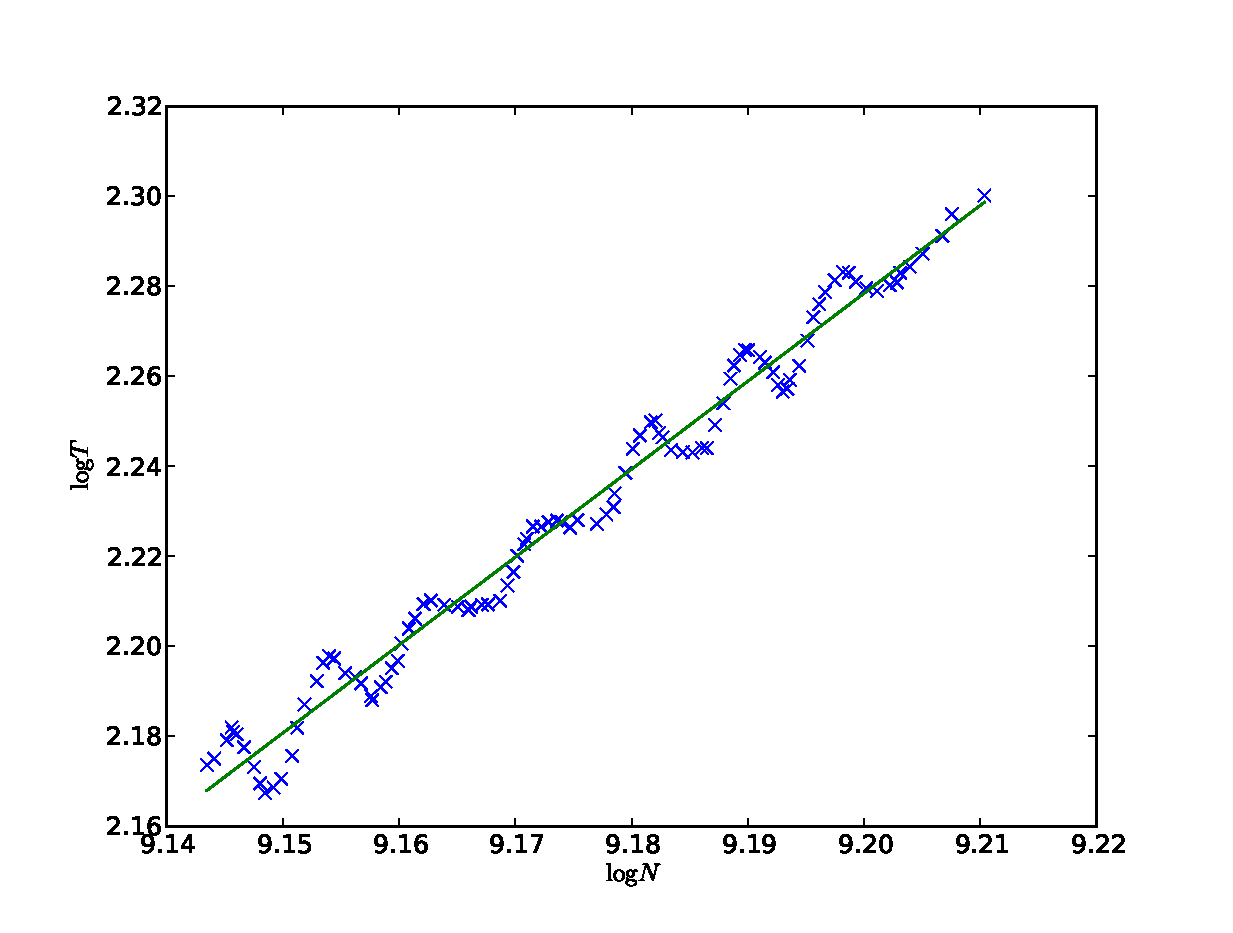
\includegraphics[width=.45\linewidth]{gfx/Evaporation/evapIP}} \quad
\subfloat[I want this to be a plot of n0 vs N.]
{\label{fig:dsmcquaderr}
\includegraphics[width=.45\linewidth]{gfx/Thermalisation/monroeIP}}
\subfloat[Not sure what plot tp put here]
{\label{fig:dsmcquaderr}
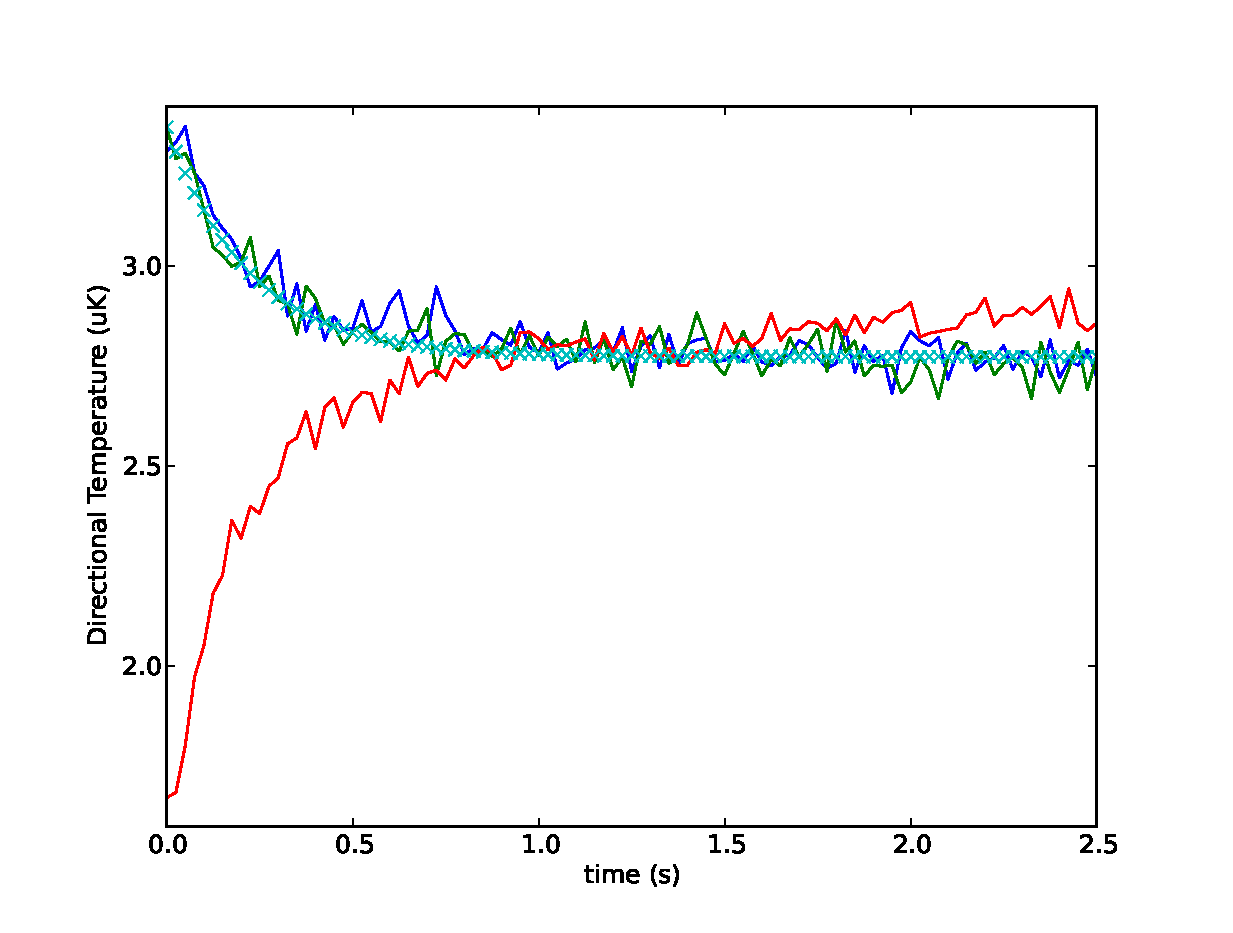
\includegraphics[width=.45\linewidth]{gfx/Thermalisation/monroeQuad}}
\caption[]{IP trap evaporation.}\label{fig:dsmccolerr}
\end{figure}

\begin{figure}[bth]
\myfloatalign
\subfloat[$\eta$ should equal ?(check the paper), here it is equal to 5 ]
{\label{fig:dsmchomoerr}
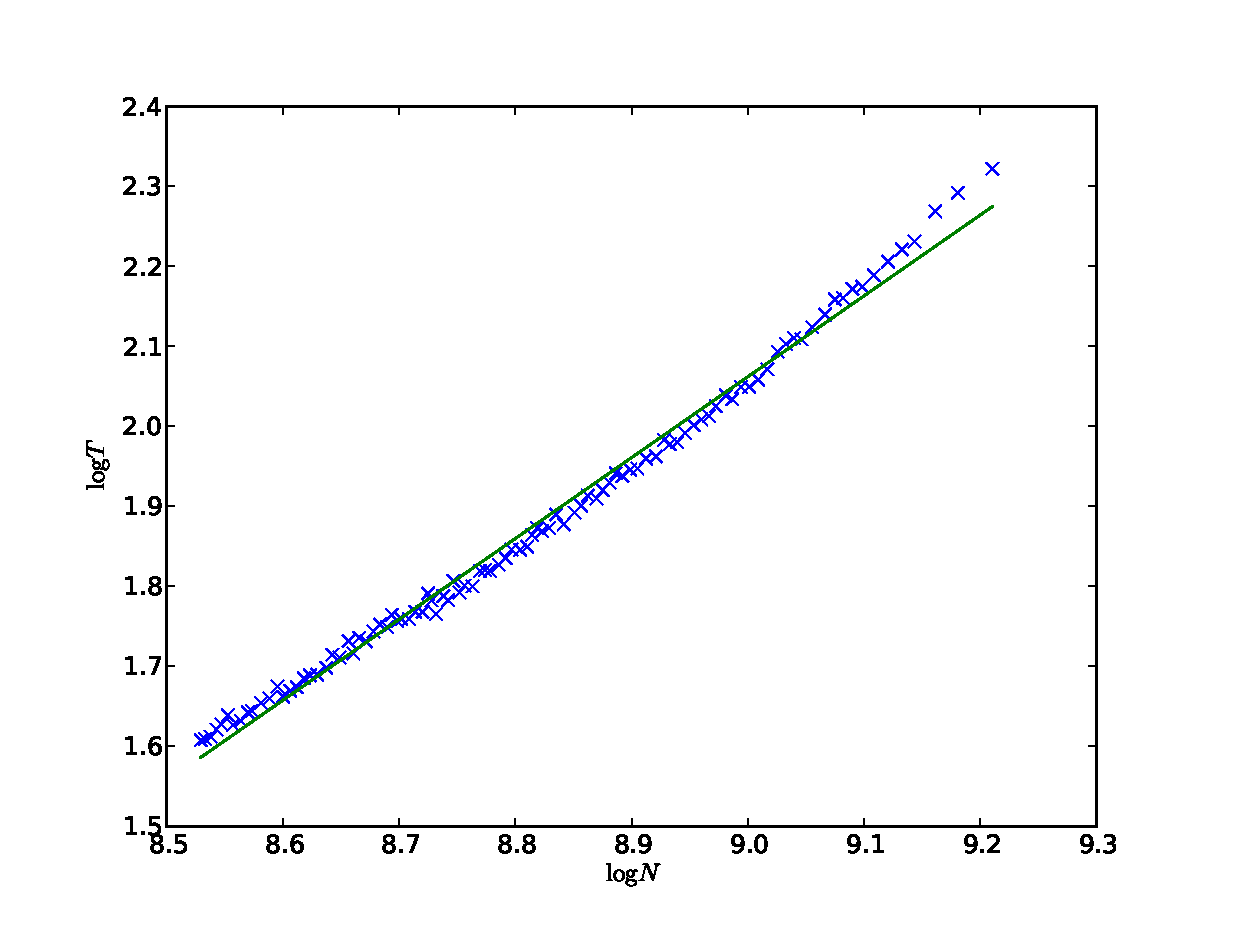
\includegraphics[width=.45\linewidth]{gfx/Evaporation/evapQuad}} \quad
\subfloat[I want this to be a plot of n0 vs N.]
{\label{fig:dsmcquaderr}
\includegraphics[width=.45\linewidth]{gfx/Thermalisation/monroeIP}}
\subfloat[Not sure what plot tp put here]
{\label{fig:dsmcquaderr}
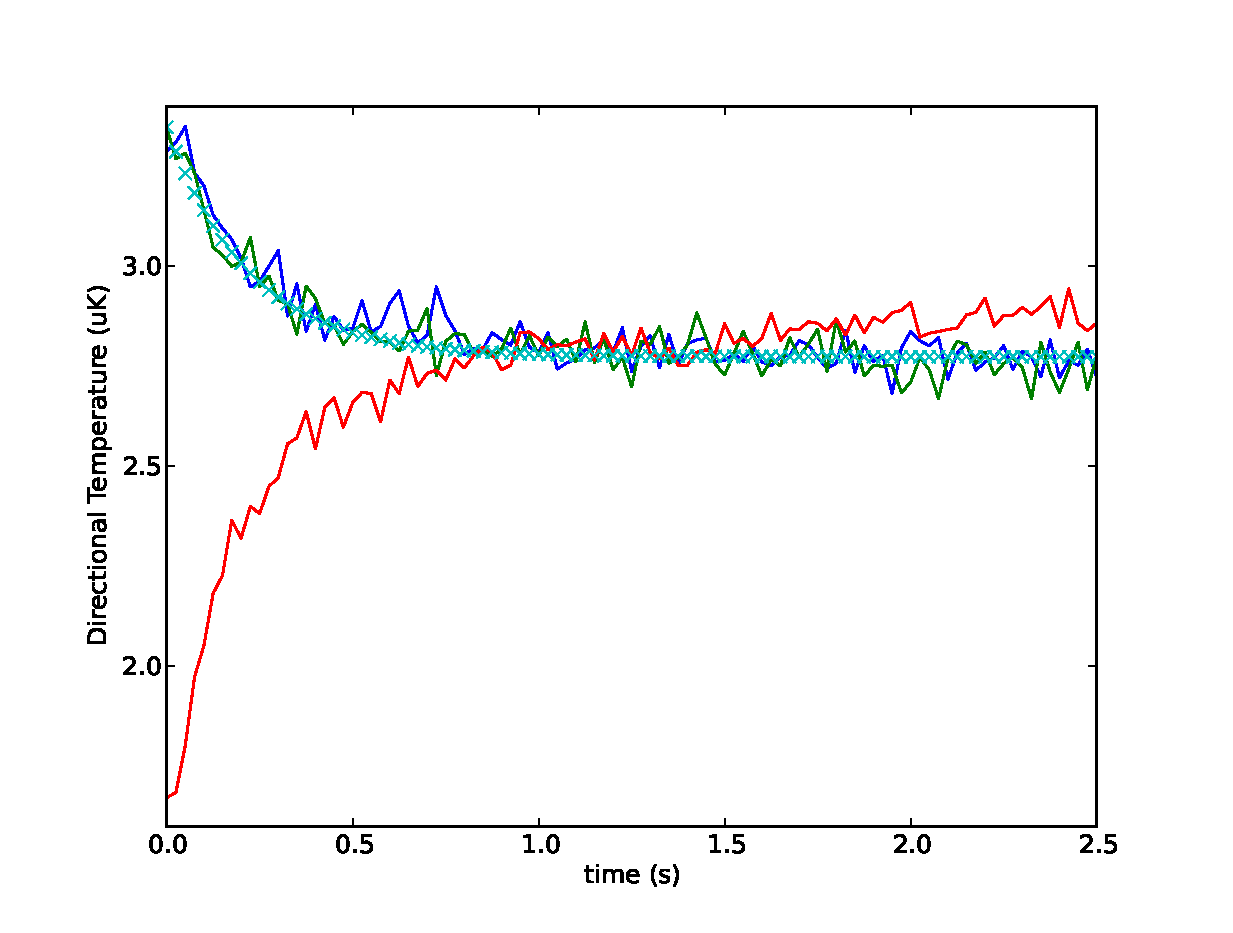
\includegraphics[width=.45\linewidth]{gfx/Thermalisation/monroeQuad}}
\caption[]{Quadrupole trap evaporation.}\label{fig:dsmccolerr}
\end{figure}

\section{Adiabaticity}

Have a look at squeezing the magnetic trap both diabaticaly and adiabatically.